Combinare una soluzione VPN sicura con una suddivisione della rete interna in compartimenti isolati sarebbe certamente ideale dal punto di vista della sicurezza.
Tuttavia, l'accesso di terze parti alla rete interna di un'organizzazione - siano essi dipendenti, clienti esterni, o altro, aggiunge delle sfide impegnative nel garantire sicurezza.
Ad esempio, se il dispositivo di un dipendente o di un cliente viene compromesso, e questa persona aveva instaurato una connessione VPN con l'azienda, coloro che hanno portato a termine l'attacco possono sfruttare il tunnel VPN come ponte per effettuare attività di ricognizione sulla rete interna dell'azienda, nonostante tutte le misure di sicurezza possibilmente implementate dall'azienda stessa.

Tuttavia, implementando una soluzione VPN moderna, è possibile monitorare il traffico, chi lo ha generato, che tipo di traffico è, e come viene usato. Tenere traccia di queste attività tramite il monitoring delle sessioni riduce i rischi, in quanto permette alle organizzazioni di identificare la sorgente del traffico sospetto e terminarlo se ritenuto opportuno.

\section{Attacchi mirati agli utenti}

Il primo step per ridurre i rischi e proteggere i dati sensibili dell'azienda è assicurarsi che tutti i dipendenti, o chiunque altro sia coinvolto nell'uso delle VPN, sappia che la sicurezza dei dati è una priorità.
Per fare questo, è necessario assicurare un'adeguata formazione a tutti loro, che copra tutti i maggiori pericoli, e le misure di difesa, che potrebbero incontrare.

È indiscutibile il fatto che alla base ci deve essere un'infrastruttura adeguata e che i dispositivi utilizzati supportino i più elevati standard di sicurezza. Infatti, i conduttori di un potenziale attacco vanno appositamente alla ricerca di, ad esempio, reti WiFI non protette, o cifrature banali da rompere.

\subsection{Furto di credenziali}
Il furto di credenziali è un tipo di crimine che consiste nel trafugare qualcosa che permette alla vittima di certificare la propria identità - ad esempio, email e password.
Una volta rubate le credenziali, colui che le ha rubate avrà gli stessi permessi e gli stessi privilegi della vittima.
Permette al ladro di resettare password, impedire alla vittima di accedere ai suoi stessi account, scaricare dati privati, ottenere accesso agli altri computer nella rete della vittima, distruggere backup, e via dicendo.

Gestire questo tipo di furti, e le loro conseguenze, dovrebbe avere altissima priorità per tutte le aziende, ma anche per i singoli utenti.

Esistono dei servizi, quali https://haveibeenpwned.com, che permettono agli utenti, inserendo il proprio indirizzo email, di verificare se sono stati coinvolti in un data breach - una divulgazione non autorizzata di dati sensibili in seguito a un attacco a una azienda. Questi servizi, che lo fanno a fin di bene, ottengono questi dati attraverso il dark web, così come lo fanno dei malintenzionati. Sapere di essere stato coinvolto in un furto di credenziali permette di prevenire un uso scorretto di esse, cambiando la password e aggiungendo misure di sicurezza più efficaci, quali ad esempio una One-Time-Password.

Le credenziali possono essere rubate sotto varie forme: hashes, tokens o anche testo in chiaro. Per trarre in inganno gli utenti, i malintenzionati spesso utilizzano la tecnica del phishing o dello spearphishing. Si tratta di soluzioni economiche ed efficienti, perché si fondando sull'interazione umana, sulla manipolazione e sull'inganno, anziché sullo sfruttamento di vulnerabilità software.

Nel caso di furto di credenziali aziendali, i criminali effettuano una ricognizione per capire chi sono le persone che posseggono i privilegi necessari a raggiungere il loro scopo, e indirizzeranno a loro i tentativi di phishing.

Alcuni modi per prevenire il furto di credenziali sono:
\begin{itemize}
    \item Autenticazione a più fattori
    \item Formazione degli utenti su come riconoscere i tentativi di Phishing
    \item Formazione degli utenti su come impostare password sicurezza
    \item Limitare l'utilizzo delle credenziali aziendali ad applicativi sicuri e controllati
    \item Mantenere aggiornati i sistemi operativi e i software utilizzati
    \item Effettuare regolarmente valutazioni sulle vulnerabilità
    \item Utilizzare strumenti di monitoring del traffico
\end{itemize}

\subsection{Social Engineering}

Con social engineering si intende quell'insieme di tecniche di manipolazione che vanno a sfruttare l'errore umano per ottenere informazioni riservate, accesso a sistemi protetti od oggetti di valore. Sono particolarmente efficaci contro utenti ingenui e/o ignoranti in materia, che non si aspettano un pericolo. Questo tipo di attacco può avvenire online, ma anche di persona o al telefono.

\subsubsection{Phishing e Spear Phishing}

Il phishing è un tipo di truffa facente parte delle tecniche di social engineering che è comunemente camuffata in email o SMS fraudolenti. La truffa consiste nel far raggiungere alla vittima la pagina di login di un sito web, dall'aspetto identica a quella del servizio di cui si vogliono rubare le credenziali, che però, anziché portare correttamente a termine il login, inoltra le credenziali al truffatore.
Tra le informazioni nel mirino dei truffatori si ha:
\begin{itemize}
    \item Username
    \item Password
    \item Indirizzo Email
    \item Residenza
    \item Numeri di carte di credito
    \item Data di nascita
\end{itemize}

Lo Spear Phishing è un caso particolare di phishing in cui il malintenzionato ha studiato la vittima e le sue abitudini. Per aumentare le possibilità di successo, infatti, includerà nel messaggio fraudolento quante più informazioni personalizzate possibili in modo da far abbassare la guardia della vittima.

Nonostante alcuni tentativi di phishing siano effettivamente ben costruiti, la maggior parte è facilmente riconoscibile.

Di seguito, alcune bandiere rosse per identificare un messaggio fraudolento:

\begin{itemize}
    \item errori ortografici e grammaticali: ad esempio, è difficile che una banca invii un messaggio non curato
    \item messaggi contenenti richieste di infromazioni personali: ad esempio richieste di credenziali per accedere a un servizio
    \item messaggi estremamente urgenti: ad esempio, un messaggio inaspettato contenente una minaccia di chiudere l'account della vittima
    \item email contenenti mittenti sospetti: ad esempio, una email proveniente da

          \texttt{john@mybankofamerica.com}, quando il dominio usuale è \texttt{@bankofamerica.com}
\end{itemize}

\subsection{Una possibile soluzione: multi-factor authentication}
A seguito di un tentativo di phishing riuscito, un malintenzionato è in possesso delle credenziali di accesso di un utente a un servizio. Se il servizio in questione è quello della VPN aziendale, egli ha accesso alla porzione di rete a cui è autorizzato ad accedere l'utente vittima.
Per diminuire drasticamente l'efficacia del phishing, uno strumento potente ed efficace è quello dell'autenticazione a più fattori.
L'autenticazione a più fattori richiede che, affinché il login abbia successo, vengano inseriti, oltre a email e password, altre ``proof of identity'', che possono essere un certificato, un'impronta digitale, una smart card, o una password monouso temporanea.

\begin{figure}[ht]
    \centering
    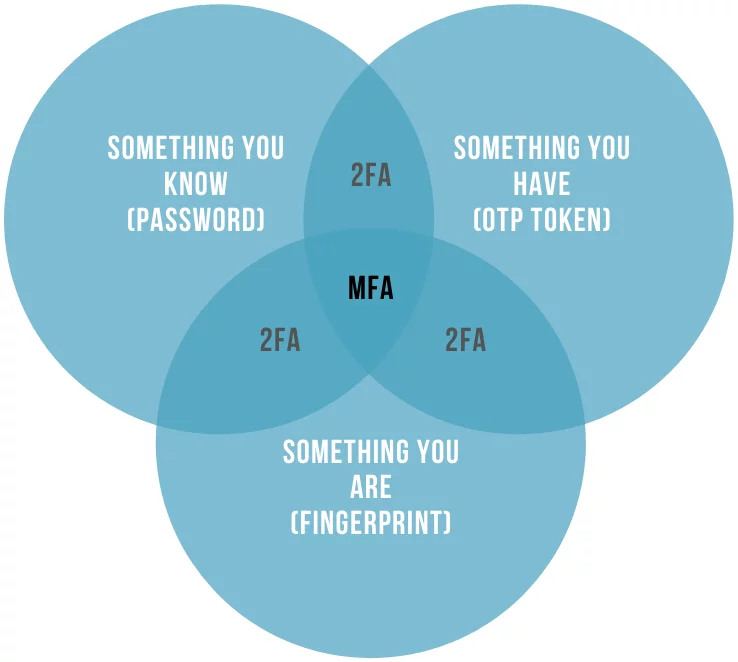
\includegraphics[width=12cm]{figure/mfa.jpeg}
    \caption{MFA}
\end{figure}

\subsubsection{Certificato}

I certificati possono essere utilizzati per autenticare sia i server VPN che i client. Generalmente, è sempre richiesto che un client che si vuole connettere sia autorizzato da un certificato.

Essi non contengono informazioni specifiche di una particolare VPN. Sono rilasciati da una Certificate Authority come prova di identità. I gateway che realizzano il tunnel VPN sono configurati in modo tale da accettare la CA che ha firmato il certificato partner come fidata. Tutti i certificati rilasciati da una CA autorizzata sono ritenuti validi, dunque si possono aggiungere e rinnovare senza alcun effetto collaterale sulla VPN. Lo stesso certificato potrebbe, anche se dipende dalla configurazione, essere utilizzato su diversi dispositivi.

I certificati riducono la manutenzione richiesta perché non devono essere cambiati così frequentemente come le Pre-Shared Keys. Tutti i certificati nascono con una data di scadenza, oltre la quale il certificato non è più valido. Dopo la scadenza, è necessario creare un nuovo certificato.

I certificati per VPN possono essere generati sia da una CA esterna che da una interna, a patto che i gateway siano configurati in modo tale da accettarla come fidata.

Come controindicazione, si ha che tutti i client VPN devono supportare l'algoritmo della CA, altrimenti è impossibile instaurare una comunicazione.


\subsubsection{Username e password}

L'autenticazione con username e password è il metodo più semplice per identificare e autenticare gli utenti. Se la password immessa dall'utente non corrisponde a quella memorizzata nel sistema, l'accesso è ovviamente negato.

La password non viene mai memorizzata in chiaro, bensì viene memorizzato il suo hash, tramite un algoritmo di hashing scelto. Un algoritmo di hash consiste in una funzione che prende un input e restituisce un output indecifrabile e incomprensibile, da cui è impossibile ricostruire l'input, se non tramite brute-force. Tuttavia, ogni volta che l'algoritmo viene eseguito con uno stesso input, l'output è sempre uguale.
Quando l'utente inserisce la password, dunque, viene calcolato l'hash e viene confrontato l'hash calcolato con quello memorizzato sul server.

Gli svantaggi consistono principalmente nel fatto che, se il numero di utenti cresce, la manutenzione diventa particolarmente complessa. Infatti, in quei casi si è soliti ricorrere a soluzioni quali l'autenticazione di Active Directory.

\subsubsection{One Time Password}
L'autenticazione a due fattori impedisce a malintenzionati di avere accesso ai sistemi della vittima utilizzando le credenziali rubate. Infatti, l'autenticazione con OTP richiede all'utente di validare la propria identificazione inserendo una password monouso temporanea (One-Time-Password).
Questa OTP viene mostrata su qualcosa che l'utente possiede (un device apposito o una applicazione sul suo smartphone) noto come \emph{authenticator}.


\section{Attacchi mirati al sistema}
Nel mirino dei malintenzionati, non c'è solo l'utente finale. Un altro punto di ingresso possibile si ottiene sfruttando le possibili vulnerabilità non mitigate presenti sui sistemi della vittima, sia essa un utente singolo o un'intera azienda.
Infatti, nessun software è privo di bug, ed essi a volte portano a falle di sicurezza, di varie gravità. Nelle situazioni più drammatiche, una falla permette a un utente non autorizzato di eseguire codice arbitrario sul sistema colpito dalla falla.

\subsection{Versione non aggiornata}
Le software house, non appena vengono a conoscenza delle falle di cui sopra, si mettono al lavoro per rilasciare un aggiornamento che chiuda la falla.
I tempi di rilascio variano, in base a diversi fattori. È in ogni caso compito dell'amministratore di sistema essere aggiornato sulle vulnerabilità che si presentano e mantenere sempre aggiornati i software in esecuzione, o trovare altri sistemi per mitigare le falle nell'attesa che venga rilasciata una patch ufficiale.
Nel caso delle soluzioni VPN in esame, esse hanno una potente arma in loro favore.
Essendo tutte e tre open source, il codice è pubblico per la sua interezza e tutti possono ispezionarlo e modificarlo.
L'idea di fondo è: più persone esperte lavorano su quel codice, più sarà facile che le vulnerabilità vengano scoperte prima che vengano utilizzate per scopi malevoli.
Inoltre, potendo inserire modifiche, la platea di sviluppatori che potenzialmente ha le conoscenze per risolvere la falla si amplia.

\subsection{Exploit di vulnerabilità zero-day}
Una vulnerabilità senza patch è tra i casi più gravi e potenzialmente difficili da gestire. Una vulnerabilità zero-day è proprio questo, una vulnerabilità conosciuta ma senza una patch disponibile.




